\documentclass[a4paper,12pt]{article}
\usepackage{../packages/coursCollege}
\newcommand{\Chapitre}{Limites}
\renewcommand{\path}{../../}

\renewcommand{\cours}{3MA1~--~EG~--~ns~--~2025-2026}
\begin{document}
\section{Activités}
\begin{activite}
	Deux fonctions de Musy
	\tcblower
\end{activite}











\begin{activite}
Introduction géométrique à la notion de limite	
	\tcblower

Vous disposez d’un stock de plaques rectangulaires au contour rigide, mesurant 1,2 mètres de large et 2 mètres de long. Pour votre prochain déménagement, vous désirez construire des cartons, ouverts vers le haut (en forme de parallélépipèdes rectangles) selon le procédé suivant : on découpe dans les quatre coins de la plaque le même carré, puis on plie les côtés et on les scotche pour former la boîte.

\hfill
\begin{minipage}[t]{0.4\textwidth}{
\vspace{0pt}
\begin{tikzpicture}[>=latex]
  % dimensions
  \def\W{4}   % correspond à 2 m
  \def\H{2.4} % correspond à 1,2 m
  \def\x{0.6} % côté du carré découpé

  % plaque avec coins découpés
  \draw (0,0) rectangle (\W,\H);
  \draw[dashed] (0,0) -- (\x,0) -- (\x,\x) -- (0,\x) -- cycle;
  \draw[dashed] (\W,0) -- (\W-\x,0) -- (\W-\x,\x) -- (\W,\x) -- cycle;
  \draw[dashed] (0,\H) -- (\x,\H) -- (\x,\H-\x) -- (0,\H-\x) -- cycle;
  \draw[dashed] (\W,\H) -- (\W-\x,\H) -- (\W-\x,\H-\x) -- (\W,\H-\x) -- cycle;

  % cotes
  \draw[<->] (0,-0.5) -- (\W,-0.5) node[midway,below]{$2\mathrm{\,m}$};
  \draw[<->] (\W+0.5,0) -- (\W+0.5,\H) node[midway,right]{$1{,}2\mathrm{\,m}$};
\end{tikzpicture}

}
\end{minipage}
\begin{minipage}[t]{0.4\textwidth}{
\vspace{0pt}
\begin{tikzpicture}[>=latex]
  % plan du carton (réseau)
  \def\W{3.4}
  \def\H{1.8}
  \def\x{0.6}

  % face centrale
  \draw (0,0) rectangle (\W,\H);
  % rabats
  \draw (0,\H) rectangle (\W,\H+\x);      % dessus
  \draw (0,-\x) rectangle (\W,0);         % dessous
  \draw (-\x,0) rectangle (0,\H);         % gauche
  \draw (\W,0) rectangle (\W+\x,\H);      % droite

  % lignes de pliage
  \draw[dashed] (0,0) -- (\W,0);
  \draw[dashed] (0,\H) -- (\W,\H);
  \draw[dashed] (0,0) -- (0,\H);
  \draw[dashed] (\W,0) -- (\W,\H);
\end{tikzpicture}
}
\end{minipage}
\hfill

Comment obtenir des cartons de volume maximal ?
\end{activite}
\begin{activite}
	\tcblower

Une population de 25\,000 individus (au temps $t=0$) croît selon la formule
\[
  N(t)
  = 25000 + 45\,t^2,
\]
où $t$ est mesuré en jours.

\begin{tasks}
  \task Calculer la vitesse moyenne à laquelle croît la population entre les instants donnés :
  \begin{multicols}{3}	
    \begin{enumerate}
      \item $t_1 = 0$ et $t_2 = 2$
      \item $t_1 = 2$ et $t_2 = 3$
      \item $t_1 = 1$ et $t_2 = 4$
      \item $t_1 = 2$ et $t_2 = 5$
    \end{enumerate}
\end{multicols}
  \task Calculer la vitesse instantanée de la croissance à l’instant $\displaystyle t = 2$.
\end{tasks}
\end{activite}

\begin{activite}
\tcblower
On considère la fonction $f$ définie par
\[
  f(x) = 2x^2 - 1.
\]

\begin{tasks}(1)
  \task Quel est le taux (moyen) de variation entre :
  \begin{multicols}{2}	
    \begin{enumerate}
      \item $(0; f(0))$ et $(2; f(2))$ ?
      \item $(0; f(0))$ et $(1; f(1))$ ?
    \end{enumerate}
  \end{multicols}
  \task Quel est le taux instantané de variation en :
  \begin{multicols}{3}	
    \begin{enumerate}
      \item $(0; f(0))$ ?
      \item $(1; f(1))$ ?
      \item $(2; f(2))$ ?
    \end{enumerate}
  \end{multicols}
  \task Que peut-on dire de la pente de la droite tangente à la courbe représentative de $f$ en :
  \begin{multicols}{3}	
    \begin{enumerate}
      \item $(0; f(0))$ ?
      \item $(1; f(1))$ ?
      \item $(2; f(2))$ ?
    \end{enumerate}
\end{multicols}
\end{tasks}

Interpréter graphiquement l’exercice.
\end{activite}

\begin{activite}{Nombre dérivé}
\tcblower
On considère la fonction \(f\) définie par
\[
  f(x)=\dfrac{1}{2x}.
\]
\begin{tasks}(1)
  \task Calculer le taux de variation de la fonction \(f\) entre deux points d’abscisses 1 et \(x\).
  \task Calculer le nombre dérivé de la fonction \(f\) en 1 et interpréter graphiquement.
\end{tasks}
\end{activite}

\begin{activite}{Toujours possible ?}
\tcblower
On considère la fonction \(f\) définie par
\[
  f(x)=\lvert x-1\rvert.
\]
\begin{tasks}(1)
  \task Représenter graphiquement cette fonction.
  \task Estimer graphiquement \(f'(2)\) et \(f'(0)\).
  \task Calculer \(f'(2)\) et \(f'(0)\).
  \task Estimer graphiquement \(f'(1)\).
  \task Calculer \(f'(1)\).
  \task Comment s’exprime graphiquement une situation de non dérivabilité ?
\end{tasks}
\end{activite}

\begin{activite}{Fonction dérivée}
\tcblower
On considère la fonction \(f\) définie par
\[
  f(x)=\dfrac{1}{2x}.
\]
\begin{tasks}(1)
  \task Calculer le taux de variation de la fonction \(f\) entre deux points d’abscisses \(a\) et \(x\).
  \task Calculer le nombre dérivé de la fonction \(f\) entre deux points d’abscisses \(a\) et \(x\). On obtient une nouvelle fonction : la dérivée de \(f\).
  \task Existe-t-il un point du graphe de \(f\) en lequel la tangente à la courbe représentative de \(f\) (ou par raccourci « à \(f\) ») soit horizontale ? Justifier et interpréter graphiquement.
  \task En quel(s) point(s) du graphe de \(f\) la pente de la tangente à \(f\) est-elle égale à \(-\dfrac{1}{12}\) ?
\end{tasks}
\end{activite}

\begin{activite}{Notations}
\tcblower
On considère la fonction \(f\) définie par
\[
  f(x)=x^2-1.
\]
\begin{tasks}(1)
  \task Déterminer la dérivée de \(f\) en \(a\).
  \task Interpréter graphiquement.
  \task Considérer \(x\) et \(x+h\) au lieu de \(a\) et \(x\) et déterminer la dérivée de \(f\) en \(x\).
\end{tasks}
\end{activite}

\begin{activite}{Équation de la tangente}
\tcblower
On considère une fonction dérivable en \((a;f(a))\) et on s’intéresse à la tangente à (la courbe représentative de) \(f\) en \((a;f(a))\). Écrire une conjecture quant à son équation, l’illustrer et la démontrer.
\end{activite}

\begin{activite}{Tangentes extérieures}
\tcblower
On considère la fonction \(f\) définie par
\[
  f(x)=\dfrac{x^4}{x+5}.
\]
\begin{tasks}(1)
  \task Déterminer les coordonnées d’un point \(P\) tel que la tangente à la courbe représentative de \(f\) au point \(P\) passe par l’origine \((0;0)\) du repère (s’il y a plusieurs solutions, les trouver toutes).
  \task Vérifier graphiquement en représentant la courbe et les tangentes trouvées.
\end{tasks}
\end{activite}


\begin{activite}{Graphiquement}
\tcblower
\begin{tasks}(1)
  \task Parmi les fonctions représentées ci-dessous, certaines sont dérivées d’une autre. Il s’agit de les retrouver :
\end{tasks}
\begin{center}
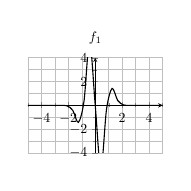
\begin{tikzpicture}[scale=0.5]
  \begin{axis}[
    title={$f_1$},
    xmin=-5, xmax=5, ymin=-4, ymax=4,
    axis lines=middle, grid=both, minor tick num=1,
    width=5cm, height=4cm
  ]
    \addplot[smooth,thick] {(32*x^3 - 24*x)*exp(-2*x^2)};
  \end{axis}
\end{tikzpicture}\quad
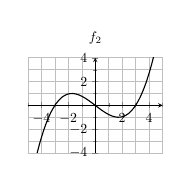
\begin{tikzpicture}[scale=0.5]
  \begin{axis}[
    title={$f_2$},
    xmin=-5, xmax=5, ymin=-4, ymax=4,
    axis lines=middle, grid=both, minor tick num=1,
    width=5cm, height=4cm
  ]
    \addplot[smooth,thick] {(x^3 - 9*x)/(6*sqrt(3))};
  \end{axis}
\end{tikzpicture}\quad
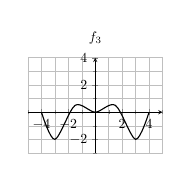
\begin{tikzpicture}[scale=0.5]
  \begin{axis}[
    title={$f_3$},
    xmin=-5, xmax=5, ymin=-3, ymax=4,
    axis lines=middle, grid=both, minor tick num=1,
    width=5cm, height=4cm
  ]
    \addplot[smooth,thick] coordinates {
      (-4,0) (-3,-2) (-1.5,0.5) (0,0) (1.5,0.5) (3,-2) (4,0)
    };
  \end{axis}
\end{tikzpicture}

\vspace{1em}

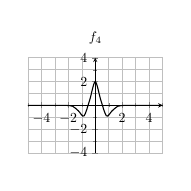
\begin{tikzpicture}[scale=0.5]
  \begin{axis}[
    title={$f_4$},
    xmin=-5, xmax=5, ymin=-4, ymax=4,
    axis lines=middle, grid=both, minor tick num=1,
    width=5cm, height=4cm
  ]
    \addplot[smooth,thick] {4*(0.5 - 2*x^2)*exp(-2*x^2)};
  \end{axis}
\end{tikzpicture}\quad
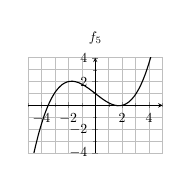
\begin{tikzpicture}[scale=0.5]
  \begin{axis}[
    title={$f_5$},
    xmin=-5, xmax=5, ymin=-4, ymax=4,
    axis lines=middle, grid=both, minor tick num=1,
    width=5cm, height=4cm
  ]
    \addplot[smooth,thick] {((x+3.5)*(x-1.5)*(x-2))/10.5};
  \end{axis}
\end{tikzpicture}\quad
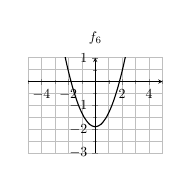
\begin{tikzpicture}[scale=0.5]
  \begin{axis}[
    title={$f_6$},
    xmin=-5, xmax=5, ymin=-3, ymax=1,
    axis lines=middle, grid=both, minor tick num=1,
    width=5cm, height=4cm
  ]
    \addplot[smooth,thick] {0.58642*(x^2 - 3.24)};
  \end{axis}
\end{tikzpicture}
\end{center}
\end{activite}


\begin{activite}{Vrai ou faux ?}
\tcblower
Vrai ou faux ? Justifier.
\begin{tasks}(1)
  \task Si \(f\) est une fonction définie sur un intervalle ouvert \(I\) et si \(a\in I\), alors \(f\) est dérivable en \(a\).
  \task Soit \(f\) la fonction définie par \(f(x)=x^2\). Si \(a\) et \(b\) sont deux nombres réels quelconques, alors le taux de variation moyen de \(f\) entre \(a\) et \(b\) est égal à \(f'\left(\dfrac{a+b}{2}\right)\).
\end{tasks}
\end{activite}

\begin{activite}{Formules de dérivation}
\tcblower
\begin{enumerate}
  \item Rappels de fonctions élémentaires dont on a calculé la dérivée à l’aide de la définition :
	  \begin{multicols}{3}	  	
    \begin{itemize}
      \item [D1] \(\mathrm{cte}'=0\)
      \item [D2] \((x)'=1\)
      \item [D3] \((ax+b)'=a\)
      \item [D4] \((x^2)'=2x\)
      \item [D5] \((ax^2+bx+c)'=2a\,x+b\)
      \item [D6] \((x^3)'=3x^2\)
      \item [D7] \(\left(\sqrt{x}\right)'=\dfrac{1}{2\sqrt{x}}\)
      \item [D8] \(\left(\tfrac{1}{x}\right)'=-\dfrac{1}{x^2}\)
    \end{itemize}
\end{multicols}
  \item Il est possible d’accélérer le calcul de \(f'(x)\), sans avoir besoin de passer par de fastidieux calculs de limites… Dans la table numérique, on trouve un formulaire de ce genre :
	  \begin{multicols}{2}	  	
    \begin{itemize}
      \item [PrD1] \([\mathrm{cte}\cdot f]'=\mathrm{cte}\cdot f'\)
      \item [PrD2] \([f+g]'=f'+g'\)
      \item [PrD3] \([f-g]'=f'-g'\)
      \item [PrD4] \([f\cdot g]'=f'\cdot g+f\cdot g'\)
      \item [PrD5] \(\left[\dfrac{1}{f}\right]'=-\dfrac{f'}{f^2}\)
      \item [PrD6] \(\left[\dfrac{f}{g}\right]'=\dfrac{f'\,g - f\,g'}{g^2}\)
      \item [PrD7] \(\left[\dfrac{\mathrm{cte}}{f}\right]'=-\mathrm{cte}\,\dfrac{f'}{f^2}\)
      \item [PrD8] \(\left[(f(x))^n\right]'=n\,[f(x)]^{n-1}\,f'(x),\;\forall n\in\mathbb{R}\)
      \item [PrD9] \(\left[g(f(x))\right]'=g'(f(x))\cdot f'(x)\)
    \end{itemize}
	  \end{multicols}
  Les utiliser pour calculer les dérivées des fonctions suivantes, en donnant les réponses sans racine au dénominateur et sans exposant numérique négatif ou fractionnaire :
    \begin{tasks}(2)
      \task \(f(x)=3x\)
      \task \(f(x)=ax+b\), avec \(a\in\mathbb{R}^*\) et \(b\in\mathbb{R}\)
      \task \(f(x)=ax^2+bx+c\), avec \(a\in\mathbb{R}^*\) et \(b,c\in\mathbb{R}\)
      \task \(f(x)=\dfrac{1}{x}\)
      \task \(f(x)=\sqrt{x^2+1}\)
      \task \(f(x)=\dfrac{1}{x^2+1}\)
      \task \(f(x)=\dfrac{\sqrt{x}}{x}\)
      \task \(f(x)=-\dfrac{2}{x^3}\)
    \end{tasks}
  \item Reprendre l’activité 1 et la résoudre en utilisant les formules de dérivation.
  \item On considère la fonction $f$ définie par \(f(x)=\dfrac{x^3}{3}-2x^2+3x\)
\begin{tasks}(1)
  \task Calculer la dérivée de \(f\).
  \task Déterminer l’équation de la tangente au graphe de \(f\) au point \((0;0)\).
  \task Trouver un autre point du graphe de \(f\) en lequel la tangente est parallèle à la précédente.
  \task Déterminer les (deux !) coordonnées des points de la courbe représentative de \(f\) en lesquels la tangente est horizontale.
  \task Utiliser vos résultats pour tracer la courbe représentative de la fonction \(f\) et les tangentes trouvées aux questions b. et c.
\end{tasks}
\end{enumerate}
\end{activite}


\begin{activite}{Une dérivée importante}
\tcblower
On considère la fonction \(f\) définie par \(f(x)=x^n\), avec \(n\in\mathbb{R}\).
\begin{tasks}(1)
  \task Calculer \(f'(x)\) pour \(n=1\), \(n=2\), \(n=0\), \(n=0,5\).
  \task Énoncer une conjecture.
  \task* La démontrer dans les cas suivants :
  \begin{multicols}{2}
    \begin{enumerate}
      \item \(n\in\mathbb{N}^*\)
      \item \(n\in\mathbb{Z}_-\)
      \item \(n\) de la forme \(\dfrac{1}{m}\) avec \(m\in\mathbb{N}^*\)
      \item \(n\in\mathbb{Q}\)
    \end{enumerate}
  \end{multicols}
\end{tasks}
\end{activite}

\begin{activite}{Relation continuité-dérivabilité}
\tcblower
\begin{tasks}(1)
\task Explorer la relation entre continuité et dérivabilité en un point.
\task Énoncer un théorème puis le démontrer.
\task Que penser de la réciproque de ce théorème ?
\end{tasks}
\end{activite}
\begin{activite}{Démonstration des formules de dérivation}
\tcblower
\begin{tasks}(1)
\task Énoncer les formules de dérivation connues comme des théorèmes en identifiant clairement hypothèses et conclusions.
\task Démontrer les théorèmes pour $\alpha \cdot f$, $f + g$, $f \cdot g$, $\dfrac{1}{f}$.
\task Démontrer le théorème pour $\dfrac{f}{g}$.
\end{tasks}
\end{activite}
\begin{activite}
	Démonstration des formules de dérivation
	\tcblower
	Énoncer et démontrer la formule de dérivation de $x^n$ comme un théorème en identifiant clairement les hypothèses et conclusions.
\end{activite}

\begin{activite}{Dérivées trigonométriques}
\tcblower
\begin{tasks}(1)
\task Représenter graphiquement la fonction sin et sa dérivée sur un même repère.
\task Quelle conjecture quant à $[\sin(x)]'$ peut-on énoncer ?
\task Démontrer ce résultat.

Indication : utiliser la formule trigonométrique $\sin(a) - \sin(b) = 2\sin\left(\dfrac{a-b}{2}\right)\cos\left(\dfrac{a+b}{2}\right)$

\task Déterminer $[\cos(x)]'$ et $[\tan(x)]'$.
\end{tasks}
\end{activite}
\begin{activite}{Une nouvelle formule de dérivation}
\tcblower
\begin{tasks}(1)
\task Comment déterminer $[\sin(x^3)]'$ ? Quelle est l'opération considérée ici ?
\task Énoncer une nouvelle formule de dérivation.
\task Déterminer :
\begin{multicols}{2}
\begin{enumerate}
\item $[\sin(4x^4-2x)]'$
\item $[\sin^4(x)]'$
\item $[\cos^2(x)]'$
\item $[\tan^4(x^4-1)]'$
\item $[\sin^4(4x^4-2x)]'$
\item $[\sin(\sin(x))]'$
\end{enumerate}
\end{multicols}
\task Quelle relation y a-t-il entre cette nouvelle formule et $\|f(x)\|^n = n[f(x)]^{n-1} \cdot f'(x), \forall n \in \mathbb{R}$
\task Énoncer une formule pour déterminer $\sqrt{f(x)}$.
\end{tasks}
\end{activite}


\begin{activite}{Théorème de Rolle}
\tcblower
On considère le théorème suivant : « Si $f: I \to \mathbb{R}$ est telle que $f$ est continue sur $[a,b]$, $f$ est dérivable sur $]a,b[$ et $f(a) = f(b)$, alors il existe au moins un nombre $c \in ]a,b[$ tel que $f'(c) = 0$ »

\begin{tasks}(1)
\task Faire un schéma pour interpréter graphiquement ce résultat.
\task Illustrer (représentation graphique, qui sont $a$, $b$ et $c$ ?) ce théorème dans les cas suivants :
\begin{enumerate}
\item $f:[-1;1] \to \mathbb{R}$ déterminée par $f(x) = x^2$
\item $f:[1;100] \to \mathbb{R}$ déterminée par $f(x) = 2$.
\item $f:[0;2] \to \mathbb{R}$ déterminée par $f(x) = x(x-2)^2$
\end{enumerate}
\task Discuter la pertinence des hypothèses.
\task * Pourquoi exige-t-on un intervalle ouvert pour la dérivabilité et un intervalle fermé pour la continuité ?
\task * Qui était Rolle ?
\task Démontrer le théorème de Rolle.
\end{tasks}
\end{activite}
\begin{activite}{Théorème des accroissements finis}
\tcblower
On considère le théorème suivant : « Si $f: I \to \mathbb{R}$ est telle que $f$ est continue sur $[a,b]$ et $f$ est dérivable sur $]a,b[$, alors il existe au moins un nombre $c \in ]a,b[$ tel que $f'(c) = \dfrac{f(b) - f(a)}{b - a}$ »

\begin{tasks}(1)
\task Faire un schéma pour interpréter graphiquement ce résultat.
\task Illustrer (représentation graphique, qui sont $a$, $b$ et $c$ ?) ce théorème dans les cas suivants :
\begin{enumerate}
\item $f:[-1;2] \to \mathbb{R}$ déterminée par $f(x) = x^2$
\item $f:[1;100] \to \mathbb{R}$ déterminée par $f(x) = 2$.
\item $f:[0;3] \to \mathbb{R}$ déterminée par $f(x) = x(x-2)^2$
\end{enumerate}
\task Discuter la pertinence des hypothèses.
\task Démontrer ce théorème.
\end{tasks}
\end{activite}
\begin{activite}{Application}
\tcblower
Trouver la ou les valeurs prévues par le théorème des AF pour la fonction $f$ définie par $f(x) = \sqrt{x}$ sur l'intervalle $[25;36]$.
\end{activite}
\begin{activite}{Corollaire du théorème des accroissements finis}
\tcblower
On considère le théorème suivant : « Soit $f$ définie sur un intervalle $I$. Alors on a :
\begin{itemize}
	\item si $f'(x) > 0, \forall x \in I$, alors $f$ est strictement croissante sur $I$
\item si $f'(x) < 0, \forall x \in I$, alors $f$ est strictement décroissante sur $I$
\item si $f'(x) = 0, \forall x \in I$, alors $f$ est constante sur $I$
\end{itemize}
\begin{tasks}(1)
\task Illustrer ce théorème.
\task À quoi est-il utile ?
\task Démontrer ce théorème.
\task Que penser de sa réciproque ?
\end{tasks}
\end{activite}


\begin{activite}{Extrema de \(f\) en \(a\) et dérivée \(f'(a)\)}
\tcblower
Nous avons vu que l’intention qui a justifié la construction de l’outil dérivée était la recherche d’extrema locaux d’une fonction donnée. Il s’agit maintenant d’aller au bout de cette démarche et d’expliciter le lien qui existe entre dérivée de \(f\) et extrema locaux de \(f'\).

\begin{tasks}(1)
  \task Donner une définition précise de la notion d’extremum global et local. Illustrer avec des exemples.
  \task Utiliser GeoGebra pour représenter des fonctions polynomiales et leur dérivée en explorant le lien supposé entre dérivée de \(f\) et extrema locaux de \(f'\).
  \task Que penser en particulier des conjectures suivantes :
    \begin{enumerate}
      \item Conjecture 1 : Si \(f : \mathbb{R}\to\mathbb{R}\) et \(a\in\mathbb{R}\) tel que \(f'(a)=0\), alors \(f\) admet un extremum local en \(a\).
      \item Conjecture 2 : Si \(f : \mathbb{R}\to\mathbb{R}\) et \(a\in\mathbb{R}\) tel que \(f\) admet un extremum local en \(a\), alors \(f'(a)=0\).
    \end{enumerate}
  \task Un point critique est un zéro de la dérivée. Les conjectures suivantes sont-elles vraies ou fausses ?
    \begin{enumerate}
      \item Conjecture 1 : Si \(f\) admet un point critique en \(a\), alors \(f'(a)=0\).
      \item Conjecture 2 : Un calcul de dérivée est toujours une indétermination de type \(\dfrac{0}{0}\).
    \end{enumerate}
\end{tasks}
\end{activite}

\begin{activite}{(Dé)croissance de \(f\) en \(a\) et signe de \(f'(a)\)}
\tcblower
Nous avons vu que l’intention qui a justifié la construction de l’outil dérivée était la recherche d’extrema locaux d’une fonction donnée. Il s’agit maintenant d’aller au bout de cette démarche et d’expliciter le lien qui existe entre dérivée de \(f\) et extrema locaux de \(f'\). Il nous faut passer à une étude plus globale du comportement de \(f\)\ldots

\begin{tasks}(1)
  \task Donner une définition précise de la notion de (dé)croissance et de (dé)croissance stricte d’une fonction. Illustrer avec des exemples.
  \task On considère le théorème suivant :

  Soit \(f\) définie sur un intervalle \(I\). Alors on a :
  \begin{itemize}
	  \item si $f'(x)>0,\ \forall\,x\in I$, alors $f$ est croissante sur $I$,
\item si $f'(x)<0,\ \forall\,x\in I$, alors $f$ est décroissante sur $I$,
\item si $f'(x)=0,\ \forall\,x\in I,$ alors $f$ est constante sur $I$.
\end{itemize}
  Illustrer ce théorème avec des exemples.
\end{tasks}
\end{activite}

\begin{activite}{Deuxième dérivée ?}
\tcblower
\begin{tasks}(1)
  \task Donner la définition de la notion de deuxième dérivée de \(f\) en illustrant avec des exemples.
  \task Que peut-on dire de la deuxième dérivée en \(a=0\) des fonctions \(f\) et \(g\) définies par
  \[
    f(x)=x^3
    \quad\text{et}\quad
    g(x)=\sqrt[3]{x}.
  \]
  \task Illustrer l’intérêt de cette notion en considérant la fonction \(f\) définie par
  \[
    f(x)=x^4+x^3+\dfrac{1}{8}.
  \]
\end{tasks}
\end{activite}

\begin{activite}{Optimisation}
\tcblower
\begin{tasks}(1)
  \task Reprendre le problème initial de déménagement et le résoudre enfin complètement.
  \task Une personne désire clôturer un terrain rectangulaire de $400~\text{m}^2$ dont un côté s’appuie sur le bord rectiligne d’une rivière, ce côté ne nécessitant pas de clôture. Déterminer les dimensions \(x\) et \(y\) du terrain pour que la longueur de la clôture soit minimale.
  \task Énoncer une méthode pour résoudre les problèmes d’optimisation.
\end{tasks}
\end{activite}

\begin{activite}{Optimisation +}
\tcblower
On considère la représentation graphique de la fonction \(f\) définie par
\[
  f(x)=\sqrt{x}-2
\]
et un point \(A(a;f(a))\) de cette courbe avec \(a<4\).

\begin{center}
	GRAPHIC
% (Graphique de la fonction et du triangle ABC ici)
\end{center}

La tangente \(t\) à \(f\) en \(A\) coupe l’axe \(O_x\) en \(B\). On s’intéresse à l’aire du triangle \(ABC\), où \(C(a;0)\) est le point de l’axe \(O_x\) d’abscisse \(a\).

\begin{tasks}(1)
  \task Montrer que l’aire du triangle \(ABC\) vaut
  \[
    a\sqrt{a} \;-\; 4a \;+\; 4\sqrt{a}.
  \]
  \task Déterminer la valeur de \(a\) pour que cette aire soit maximale.
\end{tasks}
\end{activite}

\begin{activite}{Étude de fonction}
\tcblower
\begin{tasks}(1)
  \task Étudier les fonctions définies par :
  \begin{enumerate}
    \item \(f(x)=x^3-4x\).
    \item \(f(x)=x^4+\dfrac{3}{x}+\dfrac{1}{8}\).
    \item \(f(x)=\dfrac{2x^2+2x-12}{3x-2-x^2}\).
  \end{enumerate}
\end{tasks}
\end{activite}

\begin{activite}{Étude de fonction}
\tcblower
\begin{tasks}(1)
  \task Étudier les fonctions définies par :
  \begin{enumerate}
    \item \(f(x)=\dfrac{x^2}{x+2}\).
    \item \(f(x)=\dfrac{(x-1)^3}{4(x^2+1)^2}\).
  \end{enumerate}
\end{tasks}
\end{activite}

\begin{activite}{Étude de fonction trigonométrique}
\tcblower
Étudier complètement la fonction $f$ déterminée par $f(x) = \dfrac{1}{2\sin(x)} + 2\sin(x)$.
\end{activite}

\begin{activite}{Approche physique de la notion de dérivée}
\tcblower
On appelle mouvement rectiligne un mouvement au cours duquel un objet se déplace suivant une ligne droite.

La vitesse moyenne \(v\) d’un objet qui parcourt une distance \(d\) en un temps \(t\) est
\[
  v = \dfrac{d}{t}.
\]

La vitesse de \(P\) à l’instant \(t\) (aussi appelée vitesse instantanée de \(P\) en \(t\)) est définie par
\[
  v(t) = \displaystyle\lim_{h\to 0}\dfrac{d(t+h) - d(t)}{h}.
\]

Similairement, l’accélération de \(P\) en \(t\) est définie par
\[
  a(t) = \displaystyle\lim_{h\to 0}\dfrac{v(t+h) - v(t)}{h}.
\]

\(v\) est la fonction vitesse de \(P\) et \(a\) la fonction accélération de \(P\).

On tire un projectile à la verticale avec une vitesse initiale de 120 m/s. Après \(t\) secondes, selon les lois de la physique, sa distance au sol est donnée par
\[
  r(t) = 120\,t - 5\,t^2.
\]

\begin{tasks}(1)
  \task Calculer le moment et la vitesse auxquels le projectile s’écrase au sol.
  \task Calculer l’altitude la plus élevée que le projectile atteigne.
  \task À quelle accélération le projectile est-il constamment soumis ?
\end{tasks}
\end{activite}

\begin{activite}{Dérivées et économie}
\tcblower
L’analyse est aussi un puissant outil pour résoudre les problèmes qui se présentent dans le domaine de l’économie. Quand une fonction \(f\) décrit une grandeur économique, on emploie l’adjectif « marginal » pour caractériser sa dérivée \(f'\).

À propos de la quantité \(x\) d’un bien, les économistes parlent des fonctions \(C\), \(c\), \(R\) et \(P\) pour désigner :
\begin{itemize}
  \item le coût de production \(C(x)\) de \(x\) unités ;
  \item le coût moyen de production d’une unité, défini par 
  \[
    c(x)=\dfrac{C(x)}{x};
  \]
  \item la recette \(R(x)\) de la vente de \(x\) unités ;
  \item le profit de la vente de \(x\) unités \(P\) défini par 
  \[
    P(x)=R(x)-C(x).
  \]
\end{itemize}

La variable \(x\) est traitée comme un nombre réel même si, dans ce contexte, elle ne prend le plus souvent que des valeurs entières. De plus, on a \(x\ge0\), puisque la production d’un nombre négatif d’unités n’a pas de sens !

Un fabricant de cassettes magnétiques dont les coûts mensuels fixes de production s’élèvent à CHF $8400$ et le coût de production par cassette à CHF $10$, les vend à CHF $17$ pièce :

\begin{tasks}(1)
  \task Trouver les expressions de \(C(x)\), \(c(x)\), \(R(x)\) et \(P(x)\).
  \task Quelles sont les valeurs de ces fonctions lorsque \(x=1000\) ?
  \task Combien de cassettes doit-il fabriquer pour être en équilibre financier ?
\end{tasks}

Les dérivées \(C'\), \(c'\), \(R'\) et \(P'\) des fonctions \(C,c,R\) et \(P\) portent le nom de coût marginal, coût moyen marginal, recette marginale et profit marginal, respectivement.

La valeur \(C'(x)\) représente le coût marginal associé à la production de \(x\) unités du bien. Or la dérivée est un taux de variation, donc \(C'(x)\) traduit le taux de variation du coût en fonction du nombre d’unités produites.

La même interprétation peut être donnée à propos de \(c'(x)\), \(R'(x)\) et \(P'(x)\).

Pour la fonction de coût \(C\) et \(n\) un entier positif on a, par la définition de la dérivée :
\[
  C'(n)=\displaystyle\lim_{h\to0}\dfrac{C(n+h)-C(n)}{h}.
\]
Donc, si \(h\) est petit : \(C'(n)\approx\dfrac{C(n+1)-C(n)}{h}\).

Lorsque le nombre d’unités produites est grand, les économistes considèrent que ce dernier quotient avec \(h=1\) est une bonne approximation du coût marginal, soit : \(C'(n)\approx C(n+1)-C(n)\).

Dans ces conditions, le coût marginal associé à la production de \(n\) unités d’un bien est (approximativement) le coût de la production d’une unité supplémentaire. Certaines entreprises décrivent leurs coûts de production par une fonction du type : 
\[
  C(x)=a + bx + dx^2 + kx^3.
\]
La constante \(a\) représente les frais généraux comme le loyer, le chauffage, l’éclairage qui sont indépendants du nombre d’unités produites.

Si \(b\) est le coût de production d’une unité et qu’aucun autre facteur n’intervient dans la production, alors \(bx\) représente le coût de la production de \(x\) unités du bien. Les termes \(dx^2\) et \(kx^3\) n’affecteront significativement le coût de production que pour de grandes valeurs de \(x\).

Une firme fabrique le mécanisme électronique d’un jouet. Elle estime que le coût (en CHF) de fabrication de \(x\) mécanismes est donné par
\[
  C(x)=200 + 0,05\,x + 0,0001\,x^2.
\]

\begin{tasks}(1)
	\task[d)] Quel est le coût total, le coût moyen et le coût marginal de la production de 500 unités, 1000 unités et 5000 unités ?
	\task[e)]  Comparer le coût marginal de la production de 1000 unités avec le coût de production de la mille et unième unité.
\end{tasks}

Une ébénisterie fabrique des copies de bureau de style XVIII$^\text{e}$ siècle. Elle estime le coût hebdomadaire de fabrication de \(x\) bureaux (en CHF) à 
\[
  C(x)=x^3 -3x^2 -80x +500
\]
et les vend CHF $2440$ pièce.

\begin{tasks}(1)
	\task[f)] Combien de bureaux doit-elle produire et vendre chaque semaine pour maximiser son profit ?
	\task[g)] À combien se monte ce profit hebdomadaire ?
\end{tasks}

Pour déterminer le prix de vente d’un bien qu’elle fabrique, une entreprise doit tenir compte de plusieurs facteurs. Outre le coût de production et le profit souhaité, l’entreprise doit connaître l’impact d’un changement de prix sur la demande du consommateur. Certains biens, dits de nécessité, connaissent une demande quasi constante, indépendante d’une modification du prix. Mais d’autres biens dont le prix augmente risquent fort d’être moins demandés. Généralement, une entreprise peut estimer sur la base de l’expérience passée combien d’unités seront vendues en fonction du prix unitaire pratiqué où \(p(x)\) est \(p\) une certaine fonction. À une demande de \(x\) unités correspond le prix unitaire \(p(x)\). Voilà pourquoi la fonction \(p\) est appelée fonction de demande d’un bien. La recette totale est alors le produit du nombre d’unités vendues par le prix unitaire, soit 
\[
  R(x)=x\,p(x).
\]

La demande marginale est la dérivée de \(p\).

Désignons par \(S=p(x)\) le prix de vente unitaire associé à une demande de \(x\) unités. La fonction de demande est le plus souvent décroissante, donc \(p'(x)<0\) quel que soit \(x\). Les fonctions de demande se présentent parfois implicitement par une équation qui fait intervenir \(S\) et \(x\).

La demande de \(x\) unités d’un produit est reliée à son prix de \(S\) CHF pièce par l’équation
\[
  2x + S^2 - 12000 = 0.
\]

\begin{tasks}(1)
	\task[h)] Donner l’expression de la demande, de la demande marginale, de la recette et de la recette marginale.
	\task[i)] Quelles sont les valeurs de \(x\) et de \(p(x)\) qui conduisent à une recette maximale ?
	\task[j)]  Quel est le montant de cette recette maximale ?
\end{tasks}
\end{activite}





%\newpage
%\insertexo{1M-extez}{true}{exo}{true}
%\insertexo{1M-znghn}{true}{exo}{true}
%\insertexo{1M-fazjq}{true}{exo}{true}



\subsection{derivation}
\insertexo{1M-j2esz}{true}{exo}{true}
\insertexo{1M-rqd6n}{true}{exo}{true}
\insertexo{1M-mmztw}{true}{exo}{true}
\insertexo{1M-uhfwb}{true}{exo}{true}
\insertexo{1M-sjs2h}{true}{exo}{true}
\insertexo{1M-hb4kv}{true}{exo}{true}
\insertexo{1M-g75hx}{true}{exo}{true}
\insertexo{1M-ayg94}{true}{exo}{true}
\insertexo{1M-pbjwq}{true}{exo}{true}
\insertexo{1M-5tfx9}{true}{exo}{true}
\insertexo{1M-ddnv1}{true}{exo}{true}
\insertexo{1M-nj1k9}{true}{exo}{true}
\insertexo{1M-p9k57}{true}{exo}{true}
\insertexo{1M-22t18}{true}{exo}{true}
\insertexo{1M-h2mu9}{true}{exo}{true}
\insertexo{1M-y1c7r}{true}{exo}{true}
\insertexo{1M-c6eaz}{true}{exo}{true}
\insertexo{1M-ezscr}{true}{exo}{true}
\insertexo{1M-4pfpm}{true}{exo}{true}
\insertexo{1M-bgaa8}{true}{exo}{true}

\insertexo{1M-1h2rj}{true}{exo}{true}
\insertexo{1M-bv651}{true}{exo}{true}
\insertexo{1M-1h1tt}{true}{exo}{true}
\insertexo{1M-t3pgp}{true}{exo}{true}
\insertexo{1M-r98sf}{true}{exo}{true}
\insertexo{1M-51tvf}{true}{exo}{true}
\insertexo{1M-ju5sg}{true}{exo}{true}
\insertexo{1M-ttwes}{true}{exo}{true}
\insertexo{1M-yazhe}{true}{exo}{true}
\insertexo{1M-rv1yv}{true}{exo}{true}
\insertexo{1M-vnbfx}{true}{exo}{true}
\insertexo{1M-ryapx}{true}{exo}{true}
\insertexo{1M-zeeed}{true}{exo}{true}
\insertexo{1M-gv9rr}{true}{exo}{true}
\insertexo{1M-fcxr6}{true}{exo}{true}
\insertexo{1M-8wcq9}{true}{exo}{true}
\insertexo{1M-vrkth}{true}{exo}{true}
\insertexo{1M-gmcwt}{true}{exo}{true}
\insertexo{1M-shcv8}{true}{exo}{true}
\insertexo{1M-9q8gz}{true}{exo}{true}
\insertexo{1M-xkwd5}{true}{exo}{true}
\insertexo{1M-bs74m}{true}{exo}{true}
\insertexo{1M-nv48n}{true}{exo}{true}
\insertexo{1M-pmwx1}{true}{exo}{true}
\insertexo{1M-fnj4z}{true}{exo}{true}
\insertexo{1M-bhu5u}{true}{exo}{true}
\insertexo{1M-sms7s}{true}{exo}{true}
\insertexo{1M-515q8}{true}{exo}{true}
\insertexo{1M-yn5fe}{true}{exo}{true}
\insertexo{1M-3exms}{true}{exo}{true}
\insertexo{1M-w3pgx}{true}{exo}{true}
\insertexo{1M-fg15r}{true}{exo}{true}
\insertexo{1M-2mqwc}{true}{exo}{true}
\insertexo{1M-m4mzh}{true}{exo}{true}
\insertexo{1M-wu8y4}{true}{exo}{true}
\insertexo{1M-u7dja}{true}{exo}{true}
\insertexo{1M-e1wtj}{true}{exo}{true}
\insertexo{1M-hvq58}{true}{exo}{true}
\insertexo{1M-uvgs1}{true}{exo}{true}
\insertexo{1M-7zb7h}{true}{exo}{true}
\insertexo{1M-hzaw5}{true}{exo}{true}
\insertexo{1M-uyvgj}{true}{exo}{true}
\insertexo{1M-qsgvn}{true}{exo}{true}
\insertexo{1M-kksbd}{true}{exo}{true}
\insertexo{1M-c3ghj}{true}{exo}{true}
\insertexo{1M-meks3}{true}{exo}{true}

\subsection{Limites trigonométriques}
\subsection{thm formules}
\insertexo{1M-raguk}{true}{exo}{true}
\subsection{thm importants}
\insertexo{1M-5hev4}{true}{exo}{true}
\insertexo{1M-hju27}{true}{exo}{true}
\insertexo{1M-zar8b}{true}{exo}{true}
\insertexo{1M-x5ny2}{true}{exo}{true}
\insertexo{1M-r9x4h}{true}{exo}{true}

\end{document}

